\section{Method}
\label{sec:method}
%-----------------------------------
\begin{figure}[ht]
    \centering
    \centerline{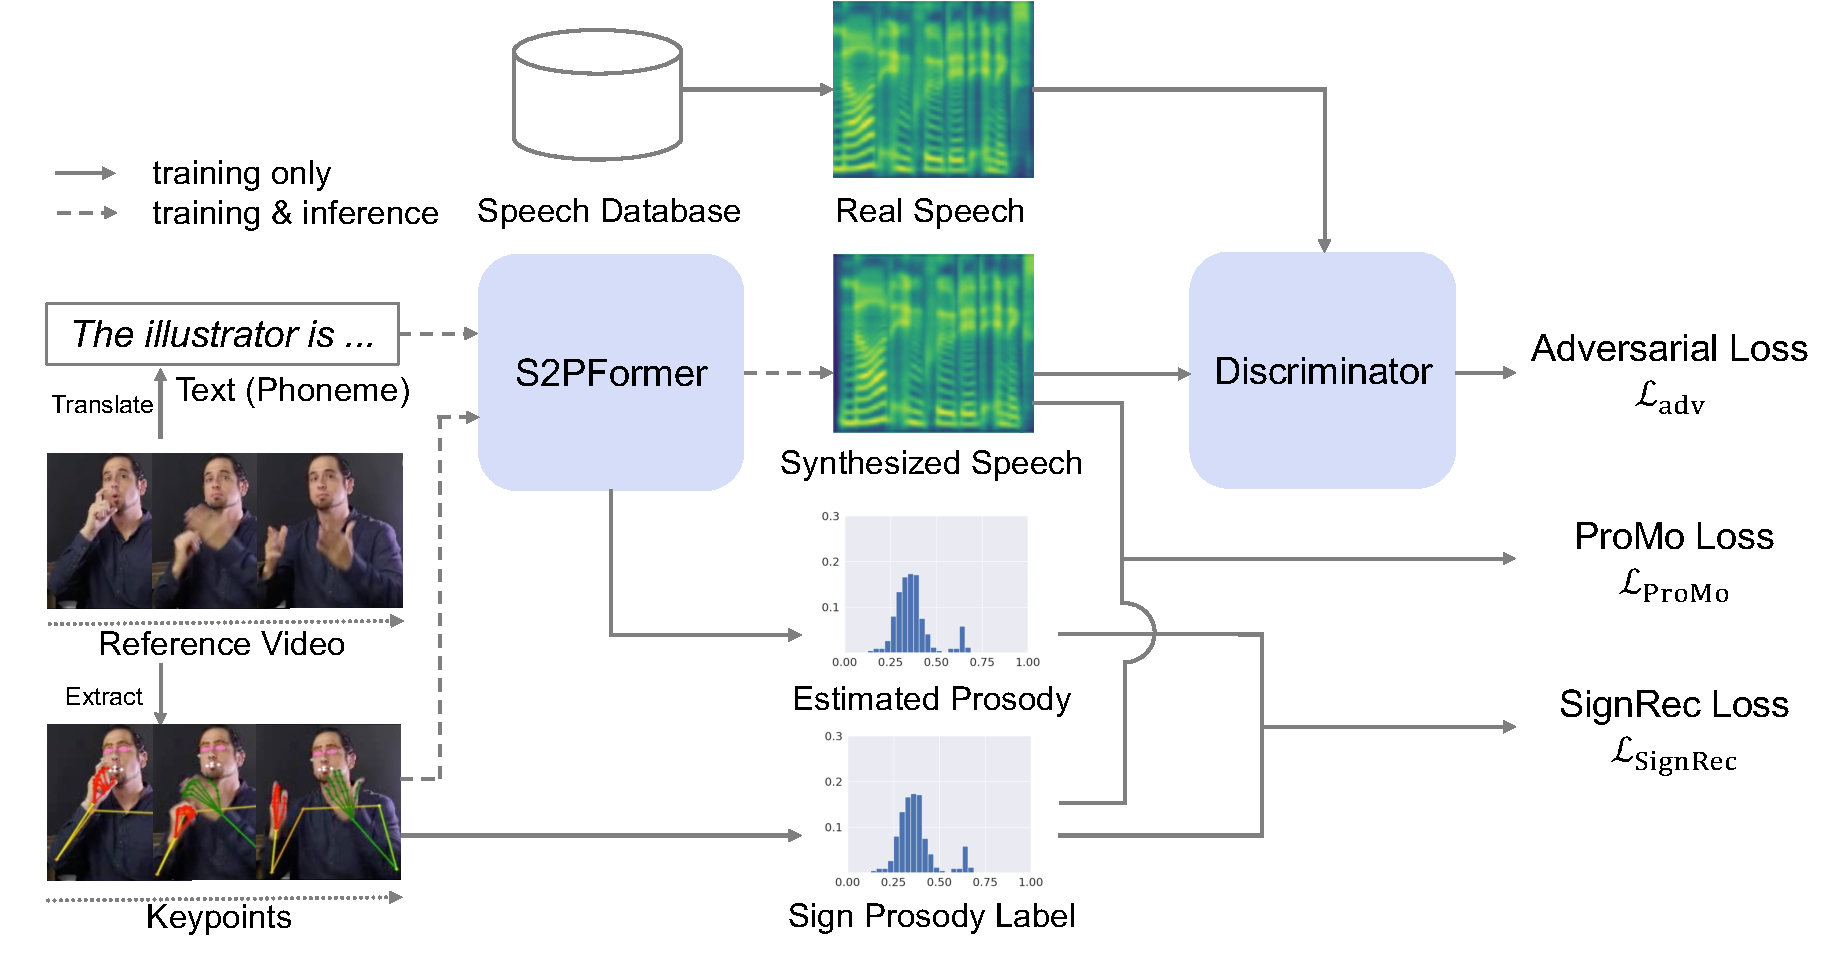
\includegraphics[width=\linewidth]{assets/concept.pdf}}
    \vspace{-2mm}
    \caption{The proposed learning framework of SignRecGAN.}
    \vspace{-4mm}
    \label{fig:overview}
\end{figure}
\manabe{
% アブストの繰り返し, 後で簡略化
We propose a novel task ``Sign-to-Speech Prosody Transfer'',
aimed at capturing the prosodic nuances conveyed
by sign language and integrating them directly
into synthesized speech.
% global prosody transferであることを定義付ける
Following prior studies of cross-lingual prosody transfer~\cite{},
our goal is to transfer global prosody of source sign into
synthesized speech.
% ↑までタスクの説明．↓フレームワークの説明
As the first baseline for this task, we propose S2PFormer.
In this paper, we use unpaired learning framework,
as in previous work,
because paired data is difficult to obtain
as we mentioned in Sec.~\ref{sec:paired_dataset}.
}

As shown in Figure~\ref{fig:overview}, 
the proposed learning framework has three main components.
First, the S2PFormer converts a pair of text and sign language video into speech that reflects sign language prosody.
Next, we introduce SignRec Loss, which reconstructs sign language prosody from the predicted speech within the S2PFormer. 
Finally, adversarial learning ensures that the synthesized speech remains realistic.
Additionally, we introduce ProMo Loss (Prosody-Motion Alignment Loss),
a regularization method that leverages prior knowledge about
how speech prosody corresponds to the movements in sign language.
% The following subsections describe S2PFormer (Sec.~\ref{sec:ts2s}) and SignRec Loss (Sec.~\ref{sec:prosody_rec}). Then, we explain ProMo Loss (Sec.~\ref{sec:PGR}).
%-----------------------------------
\subsection{S2PFormer}
\label{sec:ts2s}
\begin{figure}[t]
    \centering
    \centerline{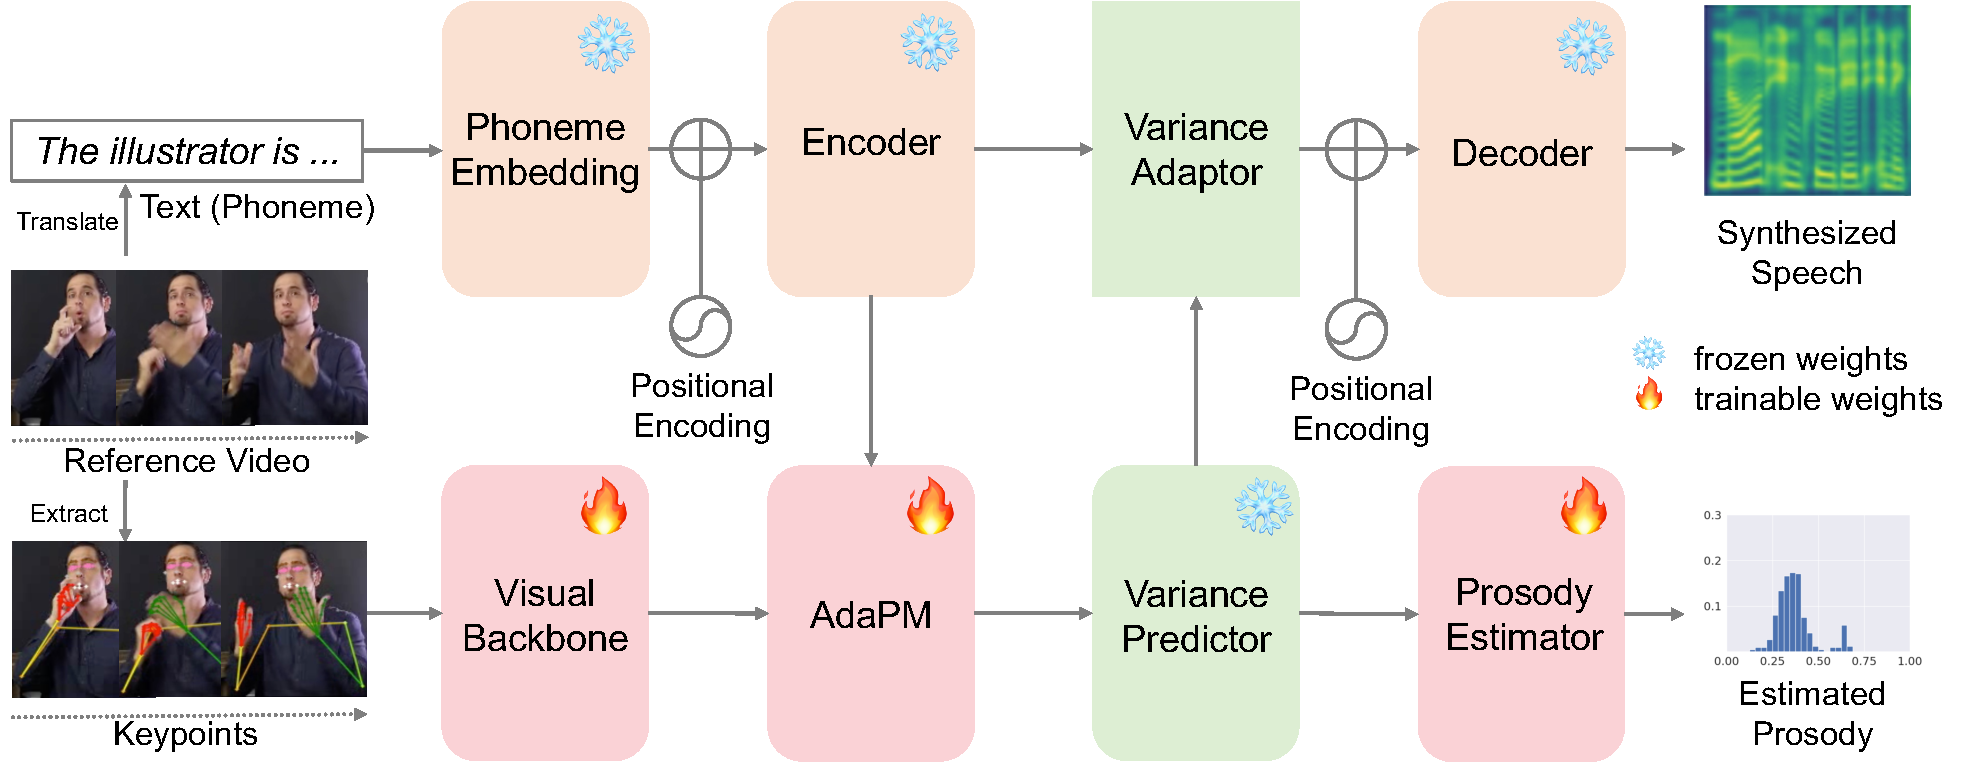
\includegraphics[width=\linewidth]{assets/ts2s.pdf}}
    \vspace{-2mm}
    \caption{The architecture of S2PFormer. S2PFormer extends FastSpeech2 by incorporating sign language information through a module called AdaPM. Specifically, the visual backbone converts sign language inputs into feature representations, which are then fed into AdaPM. Conditioned on these representations, the variance predictor estimates speech prosody parameters, which the prosody estimator uses to predict the original sign language prosody.}
    \vspace{-4mm}
    \label{fig:ts2s}
\end{figure}
The goal of S2PFormer is to effectively extract prosodic information from sign language and integrate it into speech synthesis process to synthesize speech enriched with emotion and emphasis. This module takes as input a sign language video and its corresponding translated text sequence, and outputs a mel-spectrogram that reflects the prosody of sign language.
We must preserve the original linguistic content for high-quality speech synthesis. However, linguistic and prosodic information are tightly interrelated, making it challenging to learn both simultaneously. To address this, we leverage pre-trained FastSpeech2.
We add modules to FastSpeech2 to incorporate sign language information and fine-tune only the modules.
% We augment its input with sign language information and fine-tune only the prosody-related modules.
This approach allows us to learn the relationship between sign language and speech prosody without compromising speech quality.
%-----------------------------------

\noindent
\textbf{Preliminaries of text-to-speech synthesis:}
As illustrated in Figure \ref{fig:ts2s}, a typical FastSpeech2-based module consists of four main components: Encoder, Variance Predictor, Variance Adaptor, and Decoder.
Specifically, the Encoder first converts a phoneme sequence into phoneme latent representations. Then, the Variance Predictor estimates speech prosody information, pitch, energy and duration, from the phoneme latent representations. These predicted prosodic features and phoneme latent representations are passed to the Variance Adaptor, and then processed by the Decoder to synthesize a mel-spectrogram.
In the Variance Adaptor, latent vectors corresponding to pitch and energy are first added to phoneme latent representations. Then, each element of phoneme latent representations is repeated according to predicted duration.

To incorporate and learn sign language information into speech synthesis, we introduce three additional modules: Visual Backbone, Adaptive Prosody Mixer (AdaPM), and Prosody Estimator.
These components enable the integration of sign language information into speech prosody modeling, enhancing the prosodic naturalness of the synthesized speech.

%-----------------------------------
\noindent{\textbf{Visual Backbone:}}
%-----------------------------------
Sign language is a visual language composed of both motion-based and posture-based expressions.
To extract more abstract features that capture the relationships among keypoints and their temporal dynamics, we utilize the sign language keypoint feature extraction technique employed in GloFE~\cite{lin-etal-2023-gloss}.
This Visual Backbone combines CTR-GCN~\cite{Chen_2021_ICCV}, which captures the relationships between keypoints as a graph, and MS-TCN~\cite{Liu_2020_CVPR}, which captures the relationships of keypoint positions across frames at multiple temporal resolutions. The sign language keypoints are transformed into sign language features through this backbone.

\begin{figure}[th]
    \centering
    \vspace{-2mm}
    \centerline{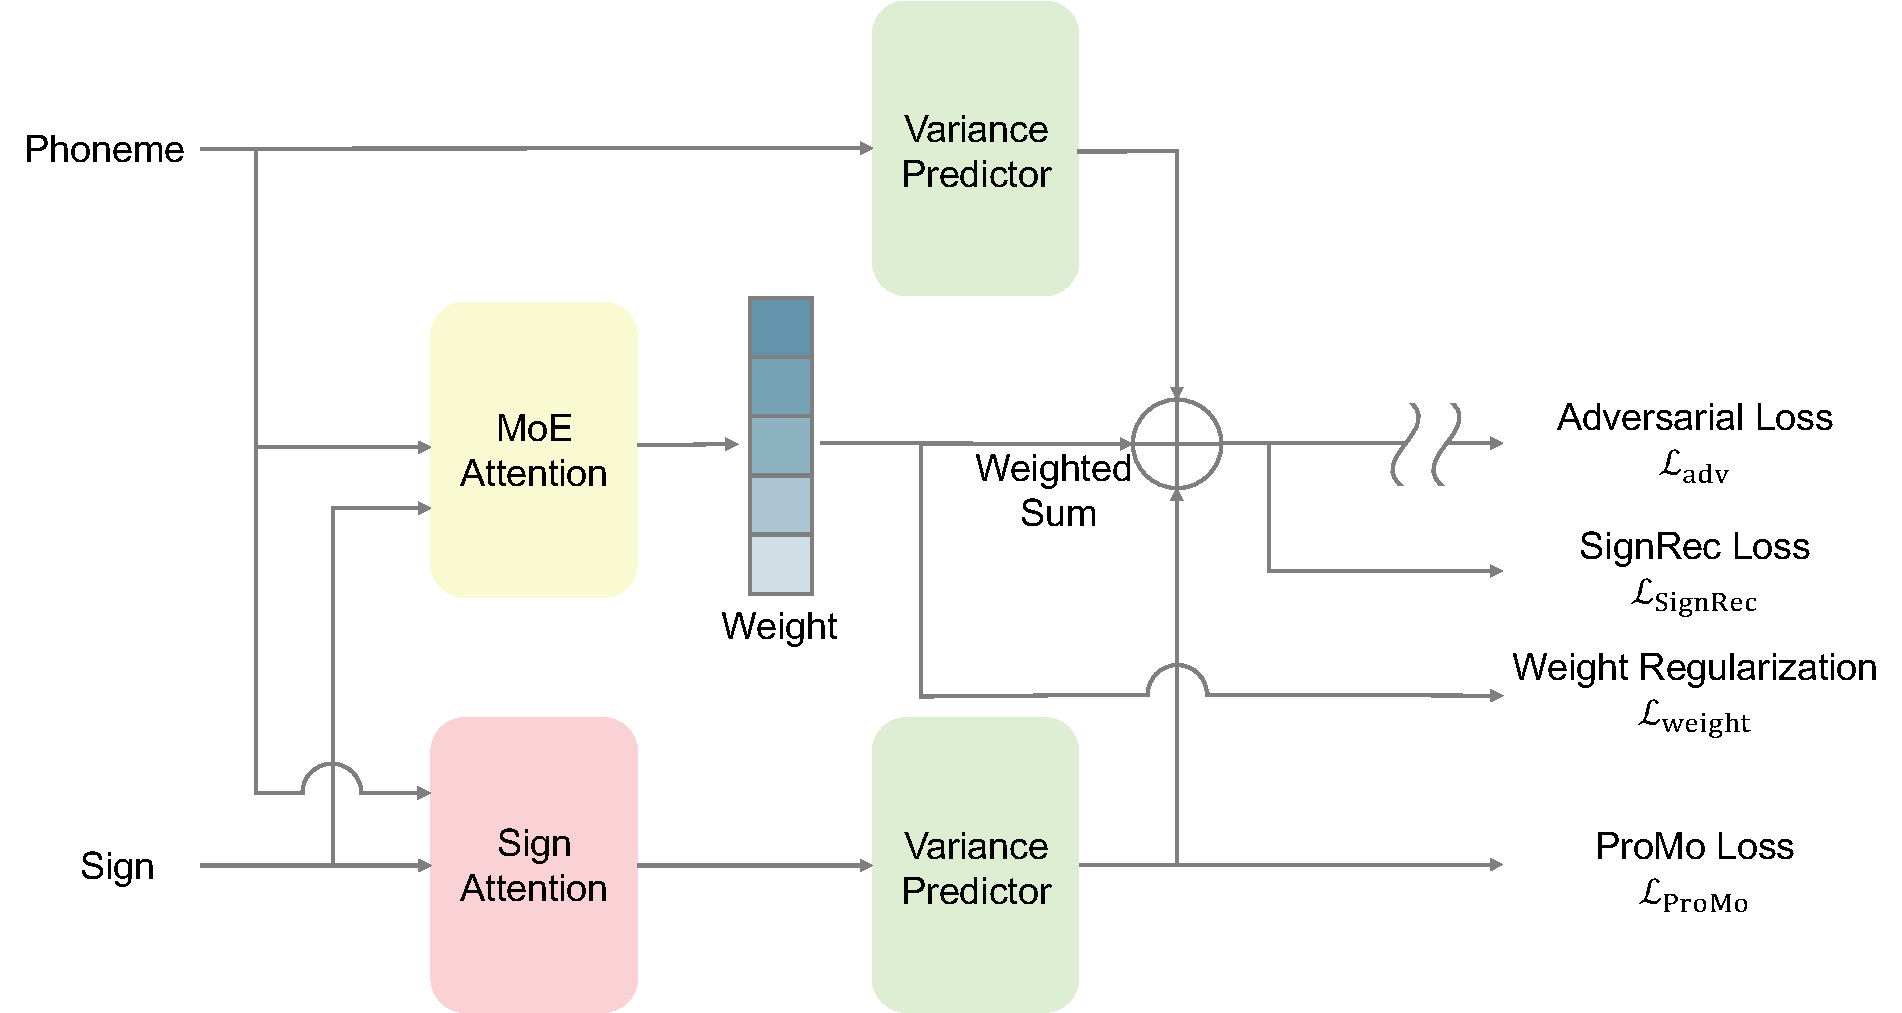
\includegraphics[width=0.8\linewidth]{assets/AdaPM.pdf}}
    \vspace{-2mm}
    \caption{Adaptive Prosody Mixer}
    \label{fig:adapm}
\end{figure}

\noindent{\textbf{Adaptive Prosody Mixer (AdaPM):}}
%-----------------------------------
To reflect sign language information in speech prosody while preserving the speech reality, we introduce AdaPM inspired by Mixture of Experts (MoE)~\cite{shazeer2017outrageouslylargeneuralnetworks}. As shown in Figure~\ref{fig:adapm}, this module mixes the variance predictions from the phoneme and the sign adaptively to balance the generative loss and sign prosody losses. Sign Attention and MoE Attention are based on the Transformer Decoder structure~\cite{NIPS2017_3f5ee243}, of which learnable parameters are initialized to 0, preventing the speech prosody from becoming noisy at the early stages of training and stabilizing adversarial learning.
Moreover, to avoid the weight for sign language features being too small, we introduce a regularization term defined as follows:
\begin{equation}
    \mathcal{L}_{\mathrm{weight}} = |1 - w_{\mathrm{sign}}|
\end{equation}
where $w_{\mathrm{sign}}$ is the mean of weight for sign language features, and $\lambda_{\mathrm{weight}}$ is a hyperparameter that controls the strength of this regularization.
%-----------------------------------
\begin{figure}[t]
    \centering
    \centerline{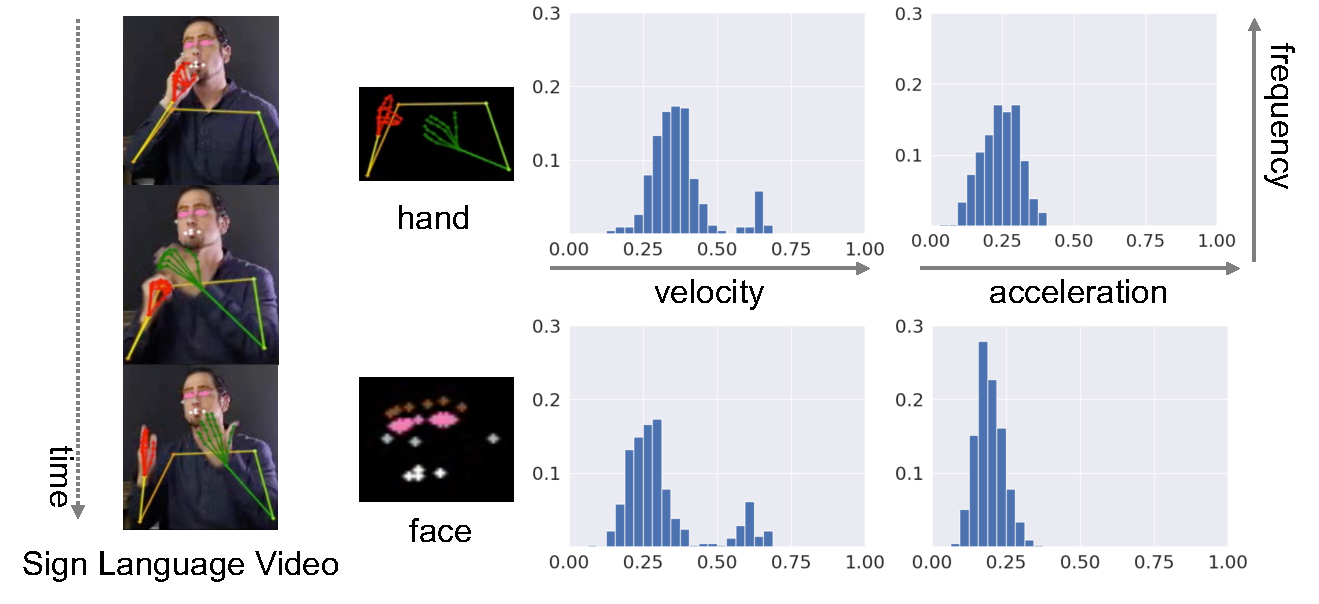
\includegraphics[width=0.8\linewidth]{assets/sign_label.pdf}}
    \vspace{-2mm}
    \caption{An example of sign language prosody labels. The histograms represent the distribution of hand and face motion information in sign language videos.}
    \vspace{-4mm}
    \label{fig:sign_label}
\end{figure}

\subsection{SignRec Loss}
\label{sec:prosody_rec}
%-----------------------------------
To ensure that the speech synthesized by S2PFormer (Sec.~\ref{fig:ts2s}) reflects sign language prosody,
we introduce the SignRec Loss, which encourages the Prosody Estimator to reconstruct sign language prosody from the resulting speech prosody.
If sign language prosody cannot be inferred at all from the speech prosody, 
it indicates there is no correlation between the two.

\noindent
{\textbf{Sign language prosody label.}} In the proposed method, sign language prosody is defined as the distribution of motion information, specifically the velocity and acceleration of representative points of the hands and face in sign language videos (see Figure~\ref{fig:sign_label}).
To create effective sign language prosody labels, we first define the sets of representative points for the hands and face, denoted as $\mathcal{H}_{\mathrm{hand}}$ and $\mathcal{H}_{\mathrm{face}}$. The velocity $v^i_t=p^i_{t+1}-p^i_t$ and acceleration $a^i_t=v^i_{t+1}-v^i_t$ are then computed for each keypoint $i$. To treat each motion information as a scalar value, the squared sum of the values for each representative point set is calculated as follows:
\begin{equation}\label{eq:V}
V^b_t=\sum_{i\in\mathcal{H}_{b}}\|v^i_t\|^2
\end{equation}
\begin{equation}\label{eq:A}
A^b_t=\sum_{i\in\mathcal{H}_{b}}\|a^i_t\|^2
\end{equation}
where $b$ is a member of the set $\{\mathrm{hand}, \mathrm{face}\}$. Let $\mathcal{M}$ be the set of pairs, each consisting of a body part and its corresponding motion information. For each $M \in \mathcal{M}$, we denote by $M_t$ the squared magnitude of the motion corresponding to $M$ at time $t$, as defined in eq.\ref{eq:V} and eq.\ref{eq:A}.
Next, the squared sums of each motion information are converted into histograms:
\begin{equation}
H_{M}(k)=\sum_{t}\iota(s_k\le M_t <s_{k+1}), s_k=k/S, 0 \le k \le S
\end{equation}
where $\iota(\bullet)$ is an indicator function, and $s_k$ represents the histogram boundaries. The sign language prosody labels are then obtained by normalizing these histograms by the sequence length $T$:
\begin{equation}
P_{M}(k)=\frac{1}{T}H_{M}(k)
\end{equation}

\noindent
{\textbf{Prosody Estimator.}}
The predicted prosody features from the Variance Predictor, pitch $\hat{p}_{\mathrm{pitch}}$ and energy $\hat{p}_{\mathrm{energy}}$, are concatenated and used as input to estimate the sign language prosody labels $\hat{P}_{M}$. The loss function for the Prosody Estimator is defined using CrossEntropy Loss as follows:
\begin{equation}\label{eq:sign_rec}
\mathcal{L}_{\mathrm{SignRec}}=-\frac{1}{4}\sum_{M \in \mathcal{M}}\sum_{k}P_{M}(k)\log\hat{P}_{M}(k).
\end{equation}
By training our model to minimize this loss, the resulting speech prosody can reconstruct 
the speed/acceleration variations and shifts in sign language motion, enabling a more faithful integration 
of sign language prosody into the synthesized speech.


%-----------------------------------
\subsection{ProMo Loss}
\label{sec:PGR}
%-----------------------------------
The learning methods described so far do not rely on paired data, meaning that how sign language prosody is reflected in speech prosody remains undetermined. To stabilize learning, we introduce cross-modal regularization terms based on prior knowledge of prosody in speech and sign language. The prior knowledge includes the correlation between the magnitude of hand movements and the energy of speech, as well as the correlation between the speed of facial movements and the pitch of speech, inspired by the studies about prosody of sign languages and spoken languages~\cite{Wilbur1999,Limousin2010}.

The ProMo Loss regularizes prosody by minimizing the L1 distance between speaker-wise standardized speech prosody $\mu_{\mathrm{energy}}, \mu_{\mathrm{pitch}}$ and video-wise standardized sign language prosody $\mu_{v, \mathrm{hand}}, \mu_{v, \mathrm{face}}$, which is defined as follows:

\begin{equation}\label{eq:pro_mo}
    \mathcal{L}_{\mathrm{ProMo}}=\max\left(\left|\mu_{\mathrm{energy}} - \mu_{v, \mathrm{hand}}\right| - c, 0\right) + \max\left(\left|\mu_{\mathrm{pitch}} - \mu_{v, \mathrm{face}}\right| - c, 0 \right)
\end{equation}
where $c$ is a margin to clip the loss to zero if the two modalities are close enough.

% Consider the case of regularizing speech prosody $m$ and sign language prosody $s$. Here, we specifically discuss regularization based on prior knowledge that $m$ and $s$ have a positive correlation. The loss function is defined by the L1 distance between the means $\mu_m$ and $\mu_s$ of each modality, expressed as $\left|\mu_m - \mu_s\right|$. Each mean is computed after standardizing the respective modality.

% \begin{equation}
%     \mathcal{L}_{\mathrm{ProMo}}=\left|\mu_m - \mu_s\right|
% \end{equation}
%-----------------------------------
\subsection{Training and Inference}
\label{sec:training_and_inference}
%-----------------------------------
In addition to the learning strategies described in Sec.~\ref{sec:prosody_rec} and Sec.~\ref{sec:PGR} for incorporating sign language prosody into speech, adversarial learning is applied to the synthesized mel-spectrograms to enhance the quality of the synthesized speech. Specifically, the discriminator $\mathcal{D}$ is trained to distinguish whether the input mel-spectrogram is real or synthesized, while the S2PFormer generator $\mathcal{G}$ is trained to deceive the discriminator into classifying synthesized speech as real speech. The adversarial learning loss is designed using the least squares loss from LSGAN~\cite{Mao_2017_ICCV}.
The loss function for the discriminator given a sign language input $X$ and a real speech mel-spectrogram $I$ is defined as follows:
\begin{equation}
    \mathcal{L}_{\mathrm{dis}} = \frac{1}{2}\left(|1 - \mathcal{D}(\mathcal{G}(X))|^2 + |\mathcal{D}(I)|^2\right)
\end{equation}

The adversarial generative loss given a sign language input $X$ is defined as follows:
\begin{equation}
    \mathcal{L}_{\mathrm{adv}} = |1 - \mathcal{D}(\mathcal{G}(X))|^2
\end{equation}

In addition to adversarial generative loss, to keep synthesized speech more natural, we introduce two regularization terms for synthesized speech: (i) regularization on the intonation, (ii) regularization on speaker likeness. The regularization on the intonation penalizes the synthesized speech if the standard deviation of the pitch and energy, $\sigma_{p}^{g}$ and $\sigma_{e}^{g}$, are smaller than those of the speech synthesized by the 2-stage method, $\sigma_{p}^{t}$ and $\sigma_{e}^{t}$. The regularization is defined as follows:
\begin{equation}
    \mathcal{L}_{\mathrm{IR}} = \max(\sigma_{p}^{g} - \sigma_{p}^{t}, 0) + \max(\sigma_{e}^{g} - \sigma_{e}^{t}, 0)
\end{equation}
The regularization on the range of pitch and energy penalizes the synthesized speech if the mean of the pitch and energy, $\mu_{p}^{g}$ and $\mu_{e}^{g}$, fall outside the speaker-specific interval, $\mu_{p}^{\mathrm{speaker}} \pm 3\sigma_{p}^{\mathrm{speaker}}$ and $\mu_{e}^{\mathrm{speaker}} \pm 3\sigma_{e}^{\mathrm{speaker}}$, where $\mu_{p}^{\mathrm{speaker}}, \mu_{e}^{\mathrm{speaker}}, \sigma_{p}^{\mathrm{speaker}}, \sigma_{e}^{\mathrm{speaker}}$ are the mean and standard deviation of pitch and energy. This constraint keeps the overall pitch and energy contours from shifting wholesale, thereby preserving the original speaker’s vocal identity instead of drifting toward a different-sounding voice. The regularization on speaker likeness is defined as follows:
\begin{equation}
    \mathcal{L}_{\mathrm{SL}} = \max(|\mu_{p}^{g} - \mu_{p}^{\mathrm{speaker}}| - 3\sigma_{p}^{\mathrm{speaker}}, 0) + \max(|\mu_{e}^{g} - \mu_{e}^{\mathrm{speaker}}| - 3\sigma_{e}^{\mathrm{speaker}}, 0)
\end{equation}
The generative loss and the regularization terms are summed up as follows:
\begin{equation}\label{eq:natural}
    \mathcal{L}_{\mathrm{natural}} = \mathcal{L}_{\mathrm{adv}} + \lambda_{\mathrm{IR}}\mathcal{L}_{\mathrm{IR}} + \lambda_{\mathrm{SL}}\mathcal{L}_{\mathrm{SL}} 
\end{equation}
where $\lambda_{\mathrm{IR}}$ and $\lambda_{\mathrm{SL}}$ are weight hyperparameters for each loss.

Finally, the generator's loss function is defined as follows:
\begin{equation}
    \mathcal{L} = \mathcal{L}_{\mathrm{natural}}+\lambda_{\mathrm{SignRec}}\mathcal{L}_{\mathrm{SignRec}}+\lambda_{\mathrm{ProMo}}\mathcal{L}_{\mathrm{ProMo}} + \lambda_{\mathrm{weight}} \mathcal{L}_{\mathrm{weight}}
\end{equation}
where $\lambda_{\mathrm{SignRec}}$ and $\lambda_{\mathrm{ProMo}}$ are weight hyperparameters for each loss.
